\chapter{Opdracht}

Om het onstaan van de opdracht te verwoorden wordt een blik geworpen op de achtergrond van het bedrijf. Shop2market is door een metormaphose gegaan in 2015 en deze opdracht is hier mede het gevolg van.

\section{Achtergrond}

Het bedrijf Shop2market is een software development bedrijf in de business-to-business sector. De organisatie helpt webwinkels online adverteren met als doelstelling de winstgevendheid van online advertenties te maximaliseren.
Shop2market is ontstaan nadat duidelijk werd dat veel bedrijven niet de technologische middelen of kennis in huis hebben om zelfstandig te kunnen starten met adverteren. Zo blijkt uit interactie met klanten dat velen vrezen voor hoge kosten.Volgens Matthijs Jorissen, komt dit door het gebrek aan transparantie en het complexe landschap dat is gecreeërd door de grootte hoeveelheid bedrijven.
Voor alsnog diende shop2market als een IT oplossing ondersteunend aan het adviesbedrijf. Het merendeel van deze klanten zijn webwinkels in het A segment. Maar omdat de integratie met een webwinkel vaak maatwerk opleverde duurde een integratie gemiddeld zes tot acht maanden. Hieruit valt ook te concluderen dat veel bedrijven niet de technologische middelen in huis hebben om zelfstandig te kunnen starten met adverteren. Ook na de integratie bleven klanten erg onderhoudsintensief. Dit hinderde de groei van Shop2market.
Daarom werd in begin 2015 gestart met de ontwikkeling van Adcurve. Met de ervaring vanuit de adviesorganisatie zijn veel processen vertaald naar functionaliteiten om een self-service applicatie mogelijk te maken. De gewenste groei is nu mogelijk doordat webwinkels gebruik maken van hetzelfde webwinkel platform zoals SEOShop, Shopify of Magento.  Dit heeft als gevolg dat Shop2market nu webwinkels in het midden en klein bedrijf op internationaal bedienent maar met een groter volume.
Webwinkels zijn nu binnen enkele minuten geïnstalleerd en kunnen hun producten gemakkelijk adverteren via zogeheten publishers. Deze kan de gebruiker zelf installeren binnen Adcurve wardoor het process geautomatiseerd word afgehaldend. Publishers zijn de bedrijven die de advertenties publiceren. De soort advertenties verschillen nogal per publisher. Denk bijvoorbeeld aan ingekochte zoekresultaten, producten op prijsvergelijkers of blogs (Affiliaties) of zelfs producten op marktplaatsen.
Zodra een gebruiker een publisher installeerd vindt er een volledige integratie plaats. Voor de webwinkel word de afkomstigheid van bezoekers en bestellingen gemeten. In combinatie met de advertentiekosten van publishers worden de nodige statistieken berekend. Met deze gegevens word de winstgevendheid van advertenties berekend.
Door de div. functionaliteiten\footnote{Denk hierbij aan datavisualiasties en beheeracties, soms ook wel "Actionable insights" genoemd.} in Adcurve kan de webwinkel zijn online marketing campagnes controleren en binnen budget houden. Dit is mogelijk doordat Adcurve een partij is tussen de webwinkel en publishers.
\pagebreak

\section{Aanleiding} % de aanleiding tot de opdracht

Het afgelopen jaar zijn de meeste basis functionaliteiten voor Adcurve ontwikkeld. Daarnaast zijn er vijf publishers geintegreerd waar voor een volledige dataintegratie plaatsvindt. Bij deze publishers worden kosten niet door ons berekend o.b.v. een percentage of vast bedrag. De kosten die in rekening zijn gebracht worden gerapporteerd en door Adcurve geïmporteerd. Omdat de belangrijkste functionaliteiten berusten op de beschikbaarheid van statistieken ligt dit proces aan de kern van het product. Helaas verloopt het importeren niet altijd zonder fouten. Het actief bewaken van datakwaliteit is hierdoor een prioriteit geworden. In de huidige situatie is dit nog lastig, doordat het berekenen van de statistieken een langdurig process is.

De huidige strategie is om meer klanten aan te trekken door meer landen en industriën te ondersteunen. Het is te verwachten dat het aantal integraties met publishers zal blijven groeien, en het probleem zal blijven groeien. Daarnaast zijn statistieken op pas s'middags beschikbaar, wat onverwachts is voor veel nieuwe gebruikers. Er is hierdoor een een toenemende wens ontstaan om de huidige oplossing te herzien. Dit moet internationale groei van Adcurve onderstuenen, en ruimte bieden om functionaliteiten betrouwbaarder en te maken.
%TODO: moet de laatste zin hierboven bij doelstellingen?

\section{Organisatie} % beschrijving van de organisatie van de opdrachtgever en de plaats van de student daarin

Shop2market is gevestigd in Hilversum en heeft tussen de 15 en 20 werknemers. De organisatie structuur kan naar de theorie van
\autocite{mintzberg} worden omschreven als een Adhocracy: “Door de innovatieve aard van projecten is een organisatie gebaat bij flexibiliteit. Een formele hiërarchische structuur werkt daardoor minder goed.” Dit is herkenbaar en valt terug te leiden naar de professionele houding die van werknemers word verwacht. Er word autonomie gegeven om zelf structuur aan te brengen wanneer dit nodig is.


\begin{figure}[h]
    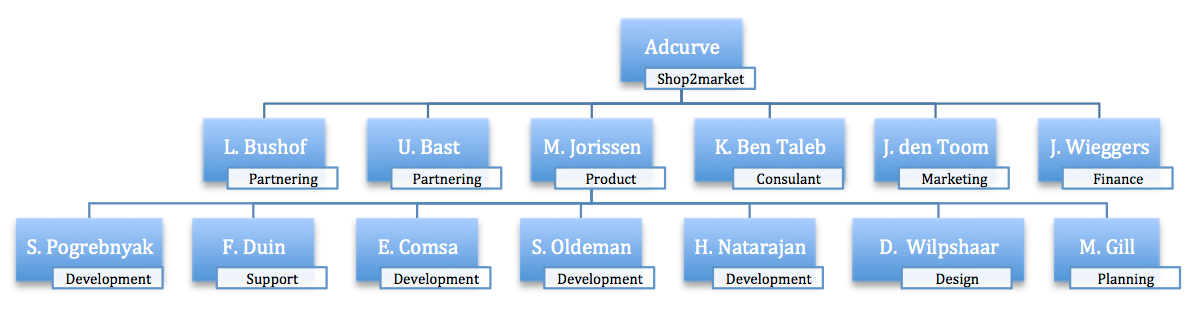
\includegraphics[width=1\textwidth]{organisation_structure.png}
    \caption{Organogram waarin de relatie tussen Shop2market en Adcurve zichtbaar is.}
    \label{fig:orgchart}
\end{figure}

\section{De kwestie} % een kwestie (aanleiding, het op te lossen probleem, de te vervullen behoefte of de te benutten kans);

Statistieken worden op dit moment dagelijks berekend voor de afgelopen dag. Dit wordt gestart rond 10:00 CET en duurt ongeveer 6 uur. Met als resultaat dat niet alle functionaliteiten actueeel zijn tijdens kantooruren.
Dit proces kan verder vertraagd raken wanneer berekeningen voor een eerdere dag opnieuw gestart zijn om een correctie uit te voeren. Het herberekenen is onderdeel van het eerder genoemde databeheer, waarbij op dit moment ook berekeningen worden gedaan voor veel databronnen die ongewijzigd blijven.

De grootste uitdaging is om altijd het meest actuele beeld te tonen over de prestaties van advertenties. Dit kan door voor kantoor uren de statistieken te berekenen. Maar niet iedere publishers stelt de kosten beschikbaar voor het importeren op het zelfde tijdstip. Webwinkel ontvangen gedurende de hele dag bestellingen of zelfs retournering van een bestelling. En de snelheid en flexibiliteit waarmee statestieken berekend kunnen worden is vaak beperkt door de gebruikte technieken of de strategische inzet van techniek. Om een actueel beel te tonene moeten berekingen opnieuw worden gestart. Maar momenteel duurt dit process gemiddeld zes uur. Het is een uitdaging om dit op slimme wijze te ontwerpen zodat dit met enige snelheid gebeurt. Dit vereist wellicht een ander algoritme bij het berekenen. Toch is het belangrijk om dezelfde resultaten uit de statistieken te berekenen.

Daarnaast is het voor de organisatie belangrijk dat een investering in een mogelijk “big data oplossing” weinig risico met zich mee brengt. Het is een uitdaging om componenten in de infrastructuur te installeren die weinig afhankelijkheden ten opzichten van elkaar hebben.


% De tijd die het duurt om statistieken te berekenen is linear gestegen met de groei in webwinkels en de hoeveelheid geinstalleerde publishers. Het is daarom de wens om de oplossing te herzien.

\section{Doelstellingen} % de doelstellingen (wat moet na afloop van het afstudeerproject zijn bereikt);

WIP: Webwinkeleigenaren maken beslissingen op actueele data uit statistieken doordat de functionaliteiten in Adcurve gebruik maken van statistieken die altijd up-to-date zijn.

Het nieuwe statistieken platform moet tijdig herstel mogelijk maken van onjuistheden. Ook moeten gebruikers functionaliteiten op basis van statistieken op tijd beschikbaar zijn voor de gebruikers. Dit moet mogelijk zijn door de snelheid waarmee berekeningen worden uitgevoerd.

Er moet een nieuwe oplossing worden ontwikkeld om statistieken te berekenen zodat functionaliteiten zoals datavisualisaties en andere functionaliteit betrouwbaar en relevant blijven.

Het nieuwe statistieken platform moet tijdig herstel mogelijk maken van onjuistheden. Ook moeten gebruikers functionaliteiten op basis van statistieken op tijd beschikbaar zijn voor de gebruikers. Dit moet mogelijk zijn door de snelheid waarmee berekeningen worden uitgevoerd.
De oplossing moet zo worden ontworpen zodat de afhankelijkheden tussen div. onderdelen in de infrastructuur minimaal zijn.
Daarnaast is het belangrijk dat de administratie van de nieuwe oplossing laagdrempelig blijft. Het is wenselijk om meer te investeren in nieuwe/ bestaande gebruikers-functionaliteiten dan in het beheer van de ondersteunende techniek.
Naast de bestaande berekeningen is het te voorzien dat er meer functionaliteiten worden ontwikkeld op basis van data analyses en dergelijken. Het is daarom wenselijk dat een oplossing voor meerdere projecten van toepassing kan zijn en dat het in gebruik nemen hiervan voor het ontwikkelteam toegankelijk is. Dit valt te verstaan onder het gebruikersgemak voor de ontwikkelaars.
Als laatste is het van uiterste belang dat de datakwaliteit wordt gewaarborgd. Door middel van data validatie zal worden gemeten of de berekeningen in de nieuwe oplossingen in dezelfde uitkomsten resulteren.


\section{Deel producten}

De opdracht is om een individueel software component te ontwikkelen. Er is daarom spraken van een product ontwikkel opdracht. Op te leveren zijn:

\begin{enumerate}
    \item Onderzoek met daarin
    \item Requirements analyse
    \item Long list en short list voor selectie van technologieën
    \item Een ontwerp voorstel o.b.v. beschikbare technologieën
    \item Een proof of concept
    \item Een statistiek platform waarop data analyses en aggregaties uitgevoerd kunnen worden.
    \item De scriptie
\end{enumerate}

% TODO: Het type opdracht kan worden omschreven als een product en ontwerp opdracht.


